\documentclass[../main.tex]{subfiles}
\begin{document}

\section{Was ist Philosophie?}
Die Liebe zur Weisheit. Ab dem 5. Jh. v. Chr. war sie eingeschränkt auf Wissen, das nicht anwendungsbezogen ist.
Heruntergebrochen lässt sich über Philosophie sagen, dass sie:
\begin{itemize}
  \item sehr allgemeine und fundamentale Fragen stellt
  \item rationale Begründungen/Argumente in den Mittelpunkt stellt
  \item sich um Fragen kümmert, die sich den empirischen Wissenschaften entziehen.
\end{itemize}

\section{Grundsätzliche Definitionen}

\subsection{Nummerische und qualitative Identität}\label{gD:numUndqualIdent}
\paragraph{Numerische Identität} beschreibt, wenn wir mit verschiedenen Begriffen über ein und dasselbe Ding reden. \\\textit{Der Morgenstern ist identisch mit dem Abendstern.} 
\paragraph{Qualitative Identität} beschreibt, wenn  zwei verschiedene Dinge sich in allen (relevanten) Aspekten gleichen. \\\textit{Diese beiden Becher sind gleich.}

\subsection{Notwendige und hinreichende Bedingungen}
\paragraph{Notwendig} ist, was unbedingt als Vorbedingung benötigt wird, damit etwas eintreten kann. \textit{Meine Schwester muss notwendigerweise weiblich sein.}
\paragraph{Hinreichend} ist, wenn aus den (erfüllten) Vorbedingungen zwingend etwas eintreten muss. \textit{Wenn eine Person weiblich ist und mein Geschwister, sind die Anforderungen, dass sie meine Schwester ist, hinreichend erfüllt.} 

\subsection{Der Ausdruck in der Sprachphilosophie}
\emph{Ausdruck} ist ein Sammelbegriff für Sätze und Satzkomponenten. 
\\Ein ganzer Text ist kein Ausdruck, ebenso wenig wie einzelne Buchstaben (Phoneme) oder die kleinsten bedeutungstragenden Einheiten (Morpheme) wie "un-" in "ungerecht".

\subsection{Gebrauch (<<use>>) vs Erwähnung (<<mention>>)}
\paragraph{Gebrauch (<<use>>)} eines Ausdruckes bedeutet, dass etwas \emph{mittels} ihm gesagt wird. Z.B. \textit{Maria ist fröhlich.}
\paragraph{Erwähnung (<<mention>>)} eines Ausdrucks bedeutet, dass man etwas \emph{über} diesen aussagt. Z.B. \textit{`Maria` hat fünf Buchstaben}. Erwähnungen können direkt (mit Anführungszeichen), indirekt (Umschreibungen) oder als sich selbst (der Ausdruck führt sich selber vor) auftreten. 

\subsection{Meinen <<mean>> vs Bedeutung haben <<mean>>}
Im Englischen benutzt man <<mean>> sowohl in Bezug auf <<bedeuten>> wie auch <<meinen>>. Gib acht darauf!

\subsection{Ontische vs proposositionale (dass-ische) Wahrheit}
\paragraph{Ontische Wahrheit} bezeichnet die Verwendung von <<wahr>> im Sinne von <<echt>>. Z.B. <<eine wahre Freundin>> ist gleich wie <<eine echte Freundin>>. 
\paragraph{Propositionale Wahrheit} bezeichnet die Verwendung von wahr im Sinne von Wahrheitsgehalt. Z.B. <<Es ist wahr, dass 2 eine Primzahl ist>>. 

\subsection{Ockhams Rasiermesser}
Ockhams Rasiermesser besagt, dass eine Theorie ontologisch sparsam sein soll. Das heisst, je weniger Kategorien/Ausnahmen sie einführt, desto besser. Im Falle von zwei Theorien, die das gleiche Verhalten erklären aber unterschiedlich funktionieren, ist diese zu bevorzugen, die mit weniger Kategorien/Ausnahmen auskommt. 

\subsection{Geschlossenheitsprinzip}
Das Geschlossenheitsprinzip besagt, dass, wenn ich weiss, dass zweiteres aus ersterem folgt, und ich weiss, dass zweiteres wahr ist, dann weiss ich auch, dass ersteres wahr ist. 

\subsection{Modus ponens}
\begin{figure}[!htb]
\centering
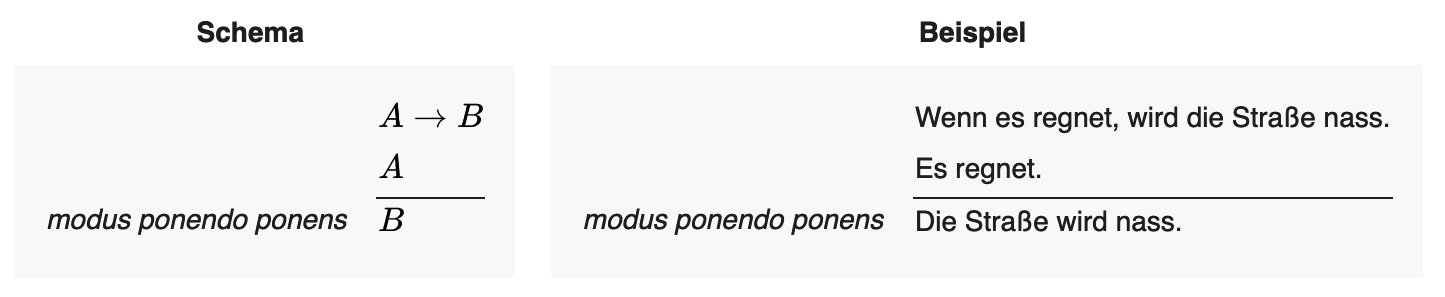
\includegraphics[width=\textwidth]{images/modus_pollens.png}
\caption{Gemäss https://de.wikipedia.org/wiki/Modus\_ponens}
\end{figure}


\subsection{Modus tollens}
\begin{figure}[!htb]
\centering
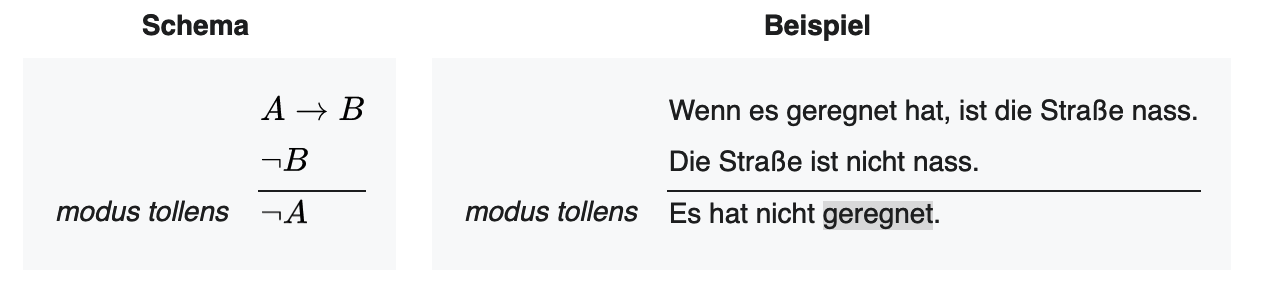
\includegraphics[width=\textwidth]{images/modus_tollens.png}
\caption{Gemäss https://de.wikipedia.org/wiki/Modus\_tollens}
\end{figure}


\subsection{Deduktive Gültigkeit}
Wenn wir die Prämissen eines Arguments akzeptieren, so können wir deren Schlussfolgerung (falls richtig durchgeführt) nicht ablehnen. 

\subsection{Intensionaler Fehlschluss}
Der intensionale (NICHT intentionale!) Fehlschluss liegt vor, wenn in einer Argumentation Referenten durch jeweils andere Referenzen gekennzeichnet werden und dies dann in der Schlussfolgerung, aufgrund des Unwissens über die Gleichheit der Bezugsobjekte, zu anderen Ergebnissen führt. 
\begin{enumerate}
	\item „Gott“ im Deutschen bezeichnet denselben „Gegenstand“ wie „Deus“ im Lateinischen oder wie „Allah“ im Arabischen.
	\item Müller glaubt an Gott.
	\item Also: Müller glaubt auch an Allah. \\
		bzw.: wenn die Konklusion 3. nicht zutrifft, kann die Prämisse 1. nicht zutreffen.
\end{enumerate}

\subsection{<<A priori>> und <<a posteriori>>}
\paragraph{a priori} bezeichnet Wissen, das unabhängig von Erfahrungen gemacht werden kann (z.B. Mathematik).
\paragraph{a posteriori} bezeichnet Wissen, das nur mittels Erfahrungen/empirischen Erkenntnissen gewonnen werden kann (z.B. dass es Planeten gibt, dass die Welt rund ist, etc.)

\subsection{synthetisch und analytisch}
\paragraph{analytisch} ist ein Satz gdw. seine Wahrheit allein an der Bedeutung der Wörter hängt.
\paragraph{synthetisch} ist ein Satz gdw. seine Wahrheit auch von der empirischen Welt, in der er geäussert wird, abhängt. 


\end{document}